\section{Przypadek Testowy 2 - Algorytm genetyczny - zależność PRD od wskaźnika mutacji}
  \subsection{Cel:}
    W tej części zostaną ze sobą porównane PRD rozwiązania algorytmu genetycznego w zależności od wskaźnika mutacji.
    \subsection{Założenia:}
    Do badania tego przypadku została wykorzystana instancja \textbf{berlin52.tsp}. Dodatkowo współczynnik selekcji został ustalony na 0.95. Ponad to wielkość populacji została ustalona na 10, liczba iteracji to 10000. Badane współczynniki mutacji \(m \in {0.05, 0.15, 0.25 ... 0.95}\). Dla każdej wielkości współczynnika mutacji test został przeprowadzony trzykrotnie.
  \subsection{Wyniki: }
  Poniższa tabela przedstawia wyniki testów, odchylenie standardowe oraz błęd standardowy.
  \begin{table}[!ht]
    \centering
    \begin{tabular}{|l|l|l|l|}
      \hline
          m & PRD & SD & SE \\ \hline
          0.05 & 48.47 & 1.54 & 0.89 \\ \hline
          0.15 & 39.30 & 16.07 & 9.28 \\ \hline
          0.25 & 36.01 & 18.63 & 10.76 \\ \hline
          0.35 & 41.24 & 19.61 & 11.32 \\ \hline
          0.45 & 38.39 & 3.52 & 2.03 \\ \hline
          0.55 & 52.92 & 24.27 & 14.01 \\ \hline
          0.65 & 60.43 & 8.97 & 5.18 \\ \hline
          0.75 & 68.26 & 13.21 & 7.62 \\ \hline
          0.85 & 70.17 & 4.90 & 2.83 \\ \hline
          0.95 & 86.56 & 6.82 & 3.94 \\ \hline
      \end{tabular}
    \caption{PRD - wyrażone w procętach [\%], SD - Odchylenie standardowe, SE - Błąd standardowy}
\end{table}
  \subsection{Wykresy: }
    \begin{figure}[H]
      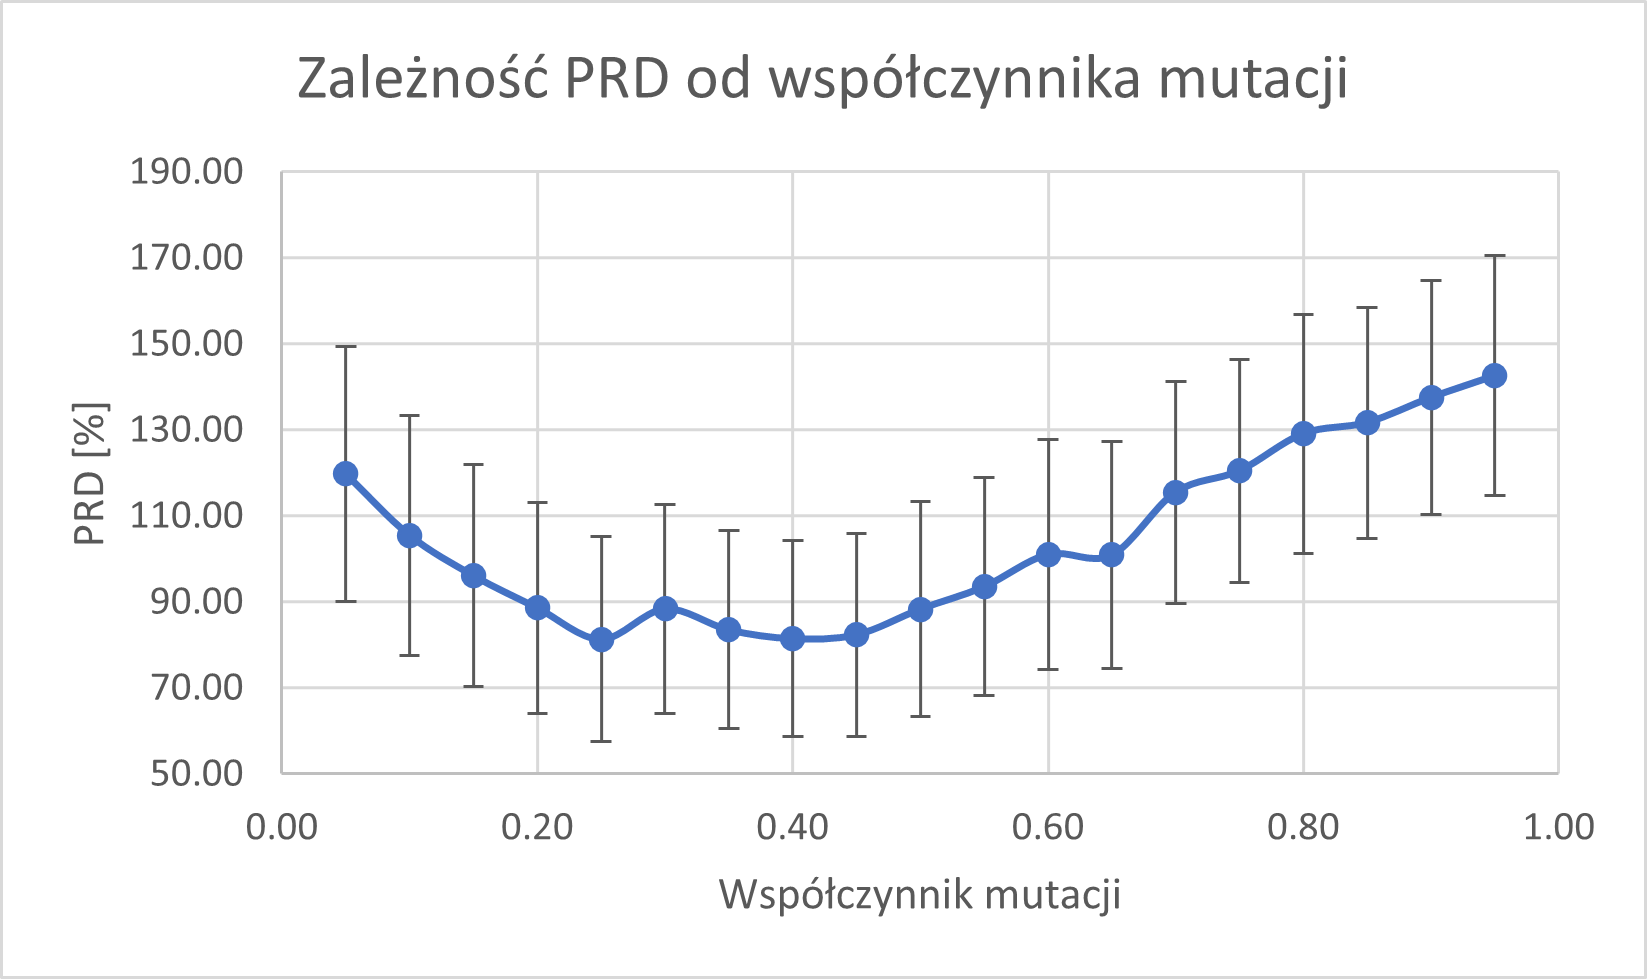
\includegraphics[scale=0.75]{chart_test_2.png}
      \centering
      \caption{zależność PRD od współczynnika mutacji}
    \end{figure}
  
    Na wykresach przedstawione są średnie wartości PRD dla badanych danych. Uśrednione wartości PRD maleją logarytmicznie, wraz ze wzrostem liczy iteracji.

    Odchylenie standardowe oraz błąd standardowy zostały obliczone według wzorów: \\
    Odchylenie standardowe:
    \[ \sigma = \sqrt{\frac{\sum_{n = 1}^{10}(\bar{x} - x_n)^2}{10}} \]
    Błąd standardowe:
    \[ \sigma_{\bar{x}} = \frac{\sigma}{\sqrt{10}} \]

  \subsection{Wnioski: }
  Zmiana współczynnik mutacji przynosi niejednoznaczne rezultaty, przez wbudowaną w mutację losowość. Można jednak zauważyć pewne zależności. Dla współczynnika mutacji 0.05 odchylenie standardowe wyników jest najmniejsze co świadczy stałości rozwiązania przy niskim poziomie mutacji. Przy szansie na mutację 0.25 algorytm osiągnął minimum w testach, jednak odchylenie standardowe było duże. W punkcie 0.45, na wykresie pojawia się minimum lokalne, w tym punkcie odchylenie standardowe znów jest niskie. po przekroczeniu 0.5 algorytm daje coraz gorsze wyniki co ma związek z częstymi mutacjami - bardziej zaczyna przypominać k-random.
